\section{Biến}
Biến được sử dụng để tham chiếm đến vị trí bộ nhớ. Biến trong Python còn được gọi là định danh và được sử dụng để lưu giá trị. Trong Python, người lập trình không cần chỉ định kiểu dữ liệu của biến biến vì Python tự động chọn kiểu dữ liệu cho phù hợp.\par
Tên biến gồm cả chữ cái và chữ số, nhưng phải bắt đầu bằng một chữ cái hoặc dấu gạch dưới. Nên sử dụng chữ cái viết thường để đặt tên cho biến. Trong Python, tên biến phân biệt chữ hoa và chữ thường.\par
\subsection{Quy cách đặt tên biến}
\begin{itemize}
	\itemsep\setlength{0em}
	\item Kí tự đầu tiên của biến bắt buộc phải là chữ cái hoặc dấu gạch dưới.
	\item Các kí tự đằng sau có thể là chữ thường, chữ hoa hoặc kí tự số.
	\item Tên biến không được chứa dấu cách hoặc các kí tự đặc biệt như *, !, @, \#, $\wedge$, \&.
	\item Tên biến không được trùng với từ khoá. Xem danh sách các từ khoá ở mục \nameref{keyword}.
\end{itemize}
Lập trình viên có thể đặt tên biến theo 3 kiểu sau đây:
\begin{itemize}
	\itemsep\setlength{0em}
	\item Kiểu lạc đà: kí tự đầu tiên viết thường, kí tự bắt đầu mỗi từ đằng sau viết hoa. Ví dụ: address, className,...
	\item Kiểu Pascal: kí tự đầu tiên của mỗi từ được viết hoa. Ví dụ: Weigth, NameOfStudent,..
	\item Kiểu con rắn:	tên biến viết thường, mỗi từ phân cách nhau bằng dấu gạch dưới. Ví dụ: check\_prime\_number,...
\end{itemize}
\subsection{Khai báo biến}
Python không bắt buộc lập trình viên phải khai báo biến trước khi sử dụng trong một ứng dụng, nó cho phép chúng ta khai báo bất cứ lúc nào người lập trình cần.\par
Người lập trình cũng không cần khai báo kiểu dữ liệu cho biến. Khi chúng ta gán dữ liệu cho nó bằng dấu "=", Python tự nhận dạng kiểu dữ liệu.\par
\textbf{Ví dụ:} \texttt{a = 10, string = "Hello world!",...}\par
Ngoài cách khai báo trên, người lập trình có thể khai báo và gán giá trị một lúc nhiều biến khác nhau. Các biến này có thể có cùng giá trị hoặc không.\par
\textbf{Ví dụ:}\\
\rule{\linewidth}{0.2mm}\par
\begin{linenumbers}
	\texttt{a = b = 5}\par
	\texttt{x, y, z = 1, 2, 3 \# x = 1, y = 2, z = 3}\par
	\texttt{\textcolor{blue}{print}(a, b)}\par
	\texttt{\textcolor{blue}{print}(x, y, z)}\par
\end{linenumbers}
\rule{\linewidth}{0.2mm}\par
\noindent
\resetlinenumber
Kết quả cho ra ở Console:\\
\rule{\linewidth}{0.2mm}\par
\begin{linenumbers}
	\texttt{5 5}\par
	\texttt{1 2 3}
\end{linenumbers}
\rule{\linewidth}{0.2mm}\par
\resetlinenumber
\newpage
\subsection{Tham chiếu đối tượng}
Người lập trình cần phải hiểu cách trình biên dịch Python hoạt động khi khai báo biến. Quá trình xử lý này có phần khác với nhiều ngôn ngữ lập trình.\par
Python là ngôn ngữ lập trình mang tính hướng đối tượng cao, đó là lý do mà mọi kiểu dữ liệu thuộc về một lớp cụ thể. Sử dụng từ khoá \texttt{"type"} để hiển thị kiểu dữ liệu của giá trị.\par
\textbf{Ví dụ:}\\
\rule{\linewidth}{0.2mm}\par
\begin{linenumbers}
	\texttt{\textcolor{blue}{print}(\textcolor{blue}{type}("Hello world!"))}\par
	\texttt{\textcolor{blue}{print}(\textcolor{blue}{type}(123))}\par
\end{linenumbers}
\rule{\linewidth}{0.2mm}\par
\noindent
\resetlinenumber
Kết quả cho ra ở Console:\\
\rule{\linewidth}{0.2mm}\par
\begin{linenumbers}
	\texttt{<class 'str'>}\par
	\texttt{<class 'int'>}
\end{linenumbers}
\rule{\linewidth}{0.2mm}\par
\resetlinenumber
Trong Python, các biến có một tên tượng trưng tham chiếu hoặc trỏ tới một đối tượng nào đó.\par
\textbf{Ví dụ}\\
\rule{\linewidth}{0.2mm}\par
	\texttt{a = 50}\\
\rule{\linewidth}{0.2mm}\par
Khi khai báo \texttt{a = 50}, biến a tham chiếu tới một đối tượng số nguyên có giá trị là 50.
\begin{figure}[h]
	\centering
	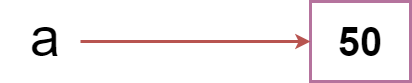
\includegraphics[width=0.7\linewidth]{img/ref1}
	\caption{Mô tả tham chiếu của biến a}
\end{figure}\par
Khi lập trình viên gán giá trị của a cho một biến b:\\
\rule{\linewidth}{0.2mm}\par
\texttt{a = 50}\par
\texttt{b = a}\\
\rule{\linewidth}{0.2mm}\par
Biến b sẽ tham chiếu tới đối tượng mà biến a đang tham chiếu tới do Python không tạo ra đối tượng mới trong trường hợp này.
\begin{figure}[h]
	\centering
	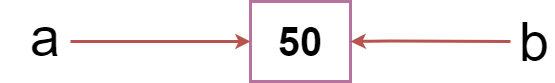
\includegraphics[width=0.7\linewidth]{img/ref2}
	\caption{Mô tả tham chiếu của biến a và b}
\end{figure}\par
Python thể hiện tính hiệu quả trong việc quản lý dữ liệu khi người lập trình gán cùng dữ liệu cho nhiều biến khác nhau.
\newpage
\subsection{Danh tính đối tượng}
Trong Python, mọi đối tượng được tạo ra đều là duy nhất. Python đảm bảo rằng không có hai đối tượng có cùng định danh. Sử dụng hàm \texttt{id()} để kiểm tra định danh của đối tượng.\par
\textbf{Ví dụ:}\\
\rule{\linewidth}{0.2mm}\par
\begin{linenumbers}
	\texttt{a = b = 1}\par
	\texttt{c = 128}\par
	\texttt{\textcolor{blue}{print}(\textcolor{blue}{id}(a))}\par
	\texttt{\textcolor{blue}{print}(\textcolor{blue}{id}(b))}\par
	\texttt{\textcolor{blue}{print}(\textcolor{blue}{id}(c))}\par
\end{linenumbers}
\rule{\linewidth}{0.2mm}\par
\noindent
\resetlinenumber
Kết quả cho ra ở Console:\\
\rule{\linewidth}{0.2mm}\par
\begin{linenumbers}
	\texttt{1824716720}\par
	\texttt{1824716720}\par
	\texttt{1824718752}
\end{linenumbers}
\rule{\linewidth}{0.2mm}\par
\resetlinenumber
Biến a và b có cùng giá trị, do đó, chúng cùng tham chiếu đến một đối tượng nên có số \texttt{id()} như nhau. Biến c có giá trị khác a và b nên số \texttt{id()} cũng khác nhau.
\newpage